%!TEX root = thesis.tex
\chapter{Results and Discussion}
\label{ch:results}

%Optimum angles and their corresponding electricity use were found for the building energy simulation for all hours of the year. For the radiation and PV evaluations, a grid-convergence study was performed and results of an optimizing angle strategy was compared to sun-tracking. The combined simulations could then be evaluated to find the most efficient overall combinations and the sensitivities of various parameters on the system performance was found.

%\section{Combined Evaluation}

By combining results for building energy simulations and PV electricity production, the overall optimum configurations can be found. Figures \ref{fig:monthly_altitude} and \ref{fig:monthly_azimuth} detail carpet-plots of the facade optimised to maximise PV generation, and minimise heating, cooling and lighting demands independently. It can be see that open configurations (light coloured) are chosen to minimise the building heating demands during the winter months and early mornings of spring and autumn. Likewise, closed configurations (dark colours) are the preferred solutions to minimise the cooling demand during the summer months. For lighting control, open positions are the optimum at all times, while the optimum altitude angles is almost exclusively at $90^{\circ}$, the azimuth angles are at $-45^{\circ}$ in the morning and at $45^{\circ}$  in the afternoon. The PV optimisation tends to choose angles that are not that extreme, corresponding to the minimization of longitudinal shading as described in section \ref{ss:compareSunTracking}. When the four optimisation cases are combined to achieve the configurations for total energy minimisation, it can be seen that there is a conflict in the summer evenings between minimising lighting and cooling demands. Likewise, we also see a conflict between heating and PV production during the winter months. The overall energy optimization including PV electricity production shows a strong tendency to follow the optimal PV production pattern. This, however changes if the building system becomes more inefficient. Less efficient heating for example, would result in configurations optimised for heating overpowering those of PV electricity generation.




\begin{figure*}
	\begin{center}
	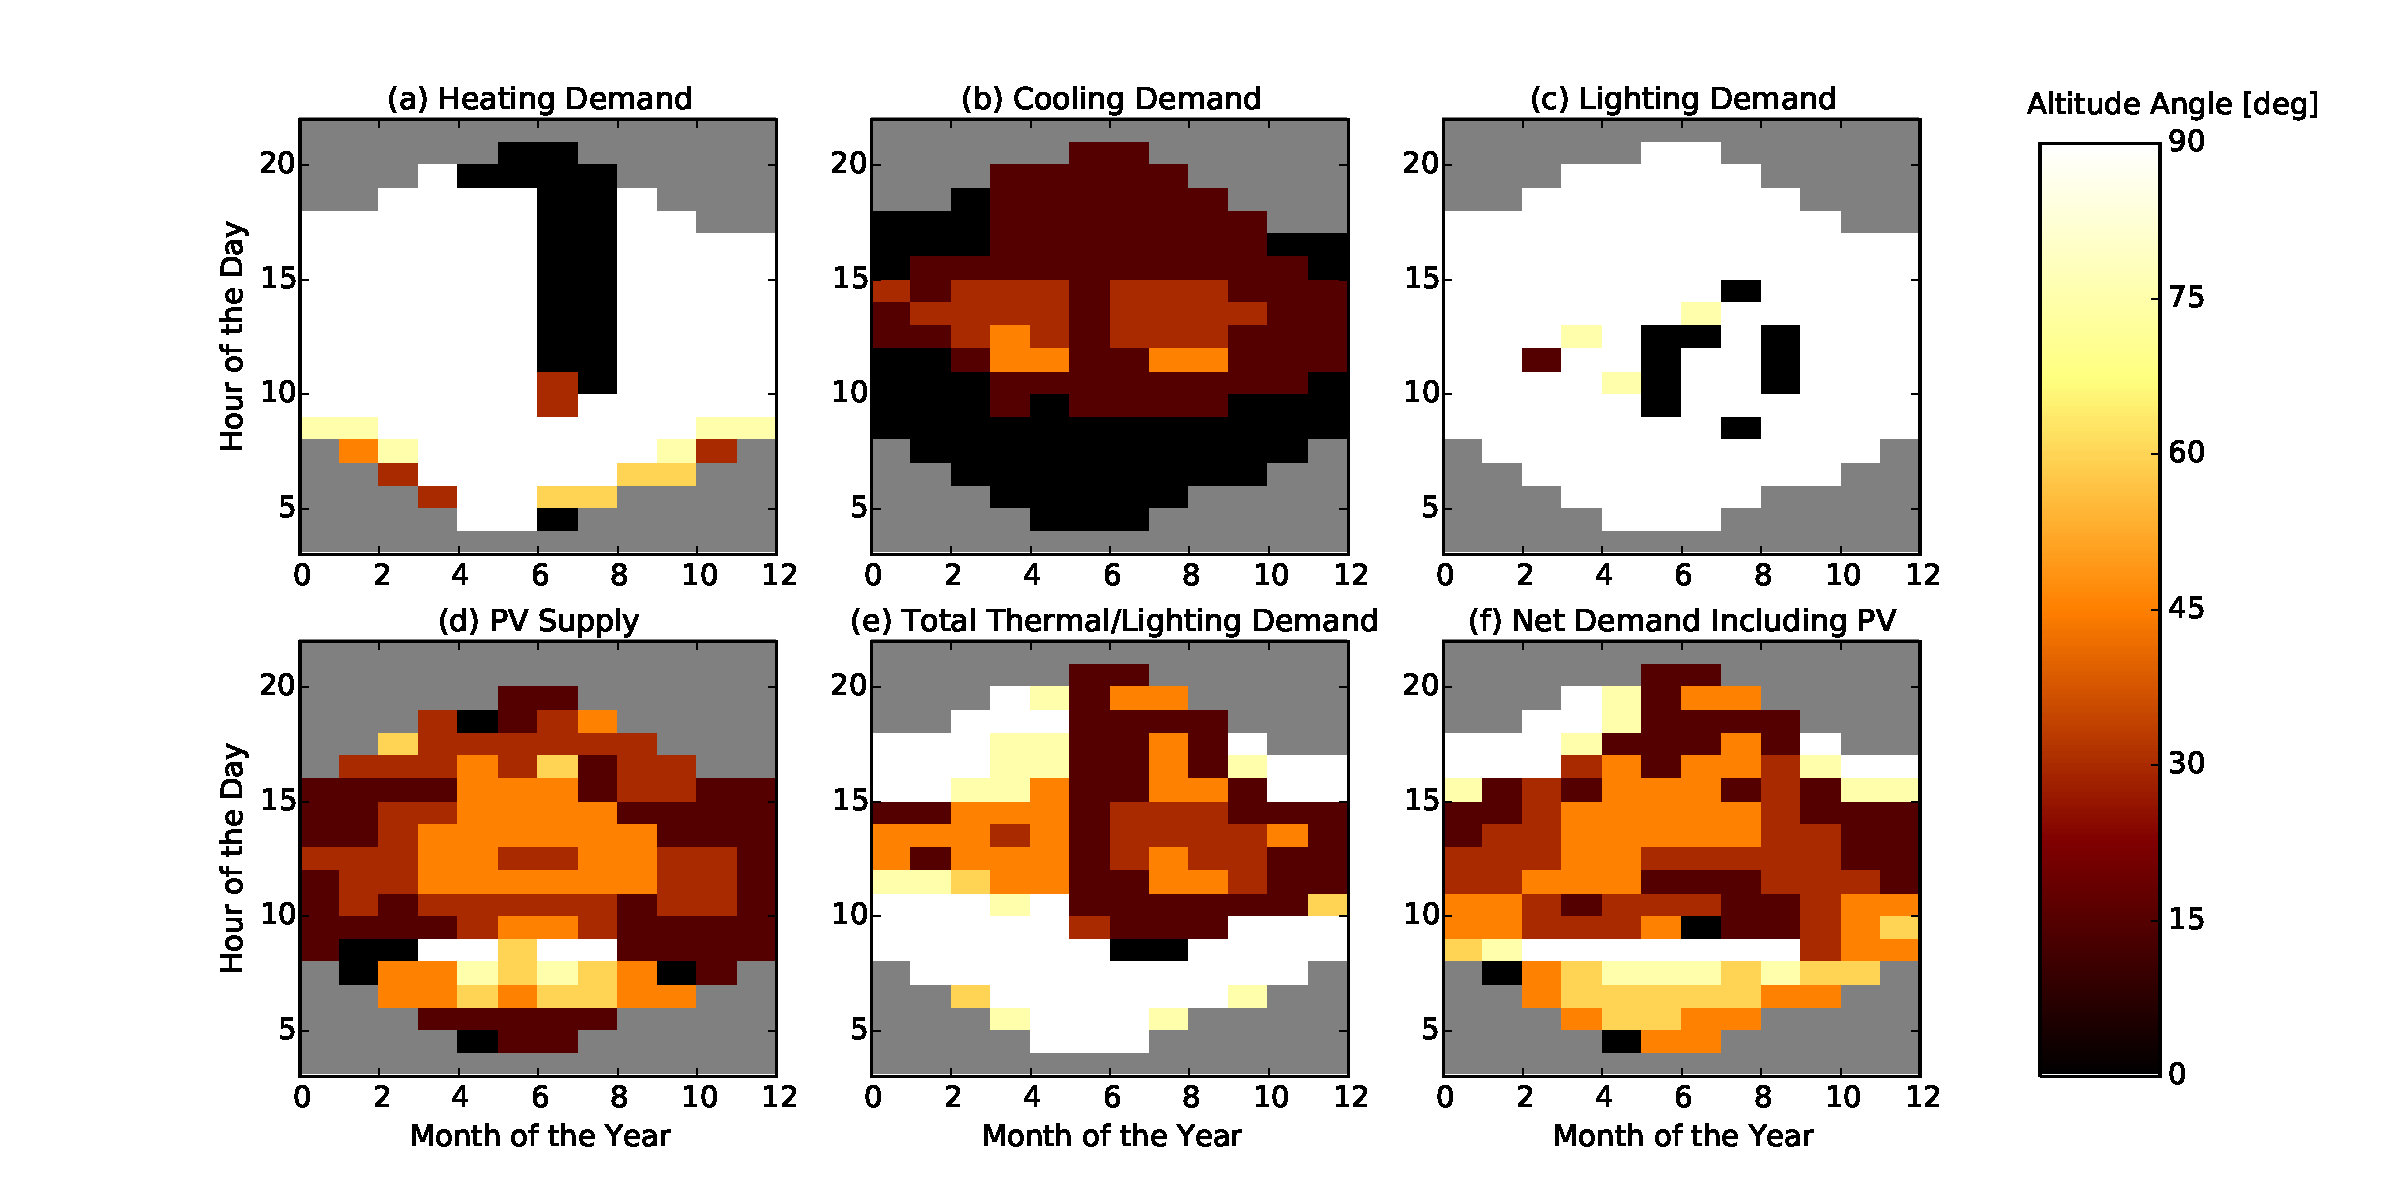
\includegraphics[width=\textwidth, trim= 0cm 0cm 0cm 0cm,clip]{monthly_altitude}
	\caption{Carpet plots detailing the optimal altitude configuration to minimise the (a) heating demand, (b) cooling demand, (c) lighting demand, and (d) maximise irradiance on PV panels. Each configuration is represented by an angle of orientation around the x-axis (Altitude) and y-axis (Azimuth) as seen in the legend. Figure (e) details the combinations for optimum building thermal management without PV production. (f) also includes the PV production}
	\label{fig:monthly_altitude}
	\end{center}
\end{figure*}

\begin{figure*}
	\begin{center}
	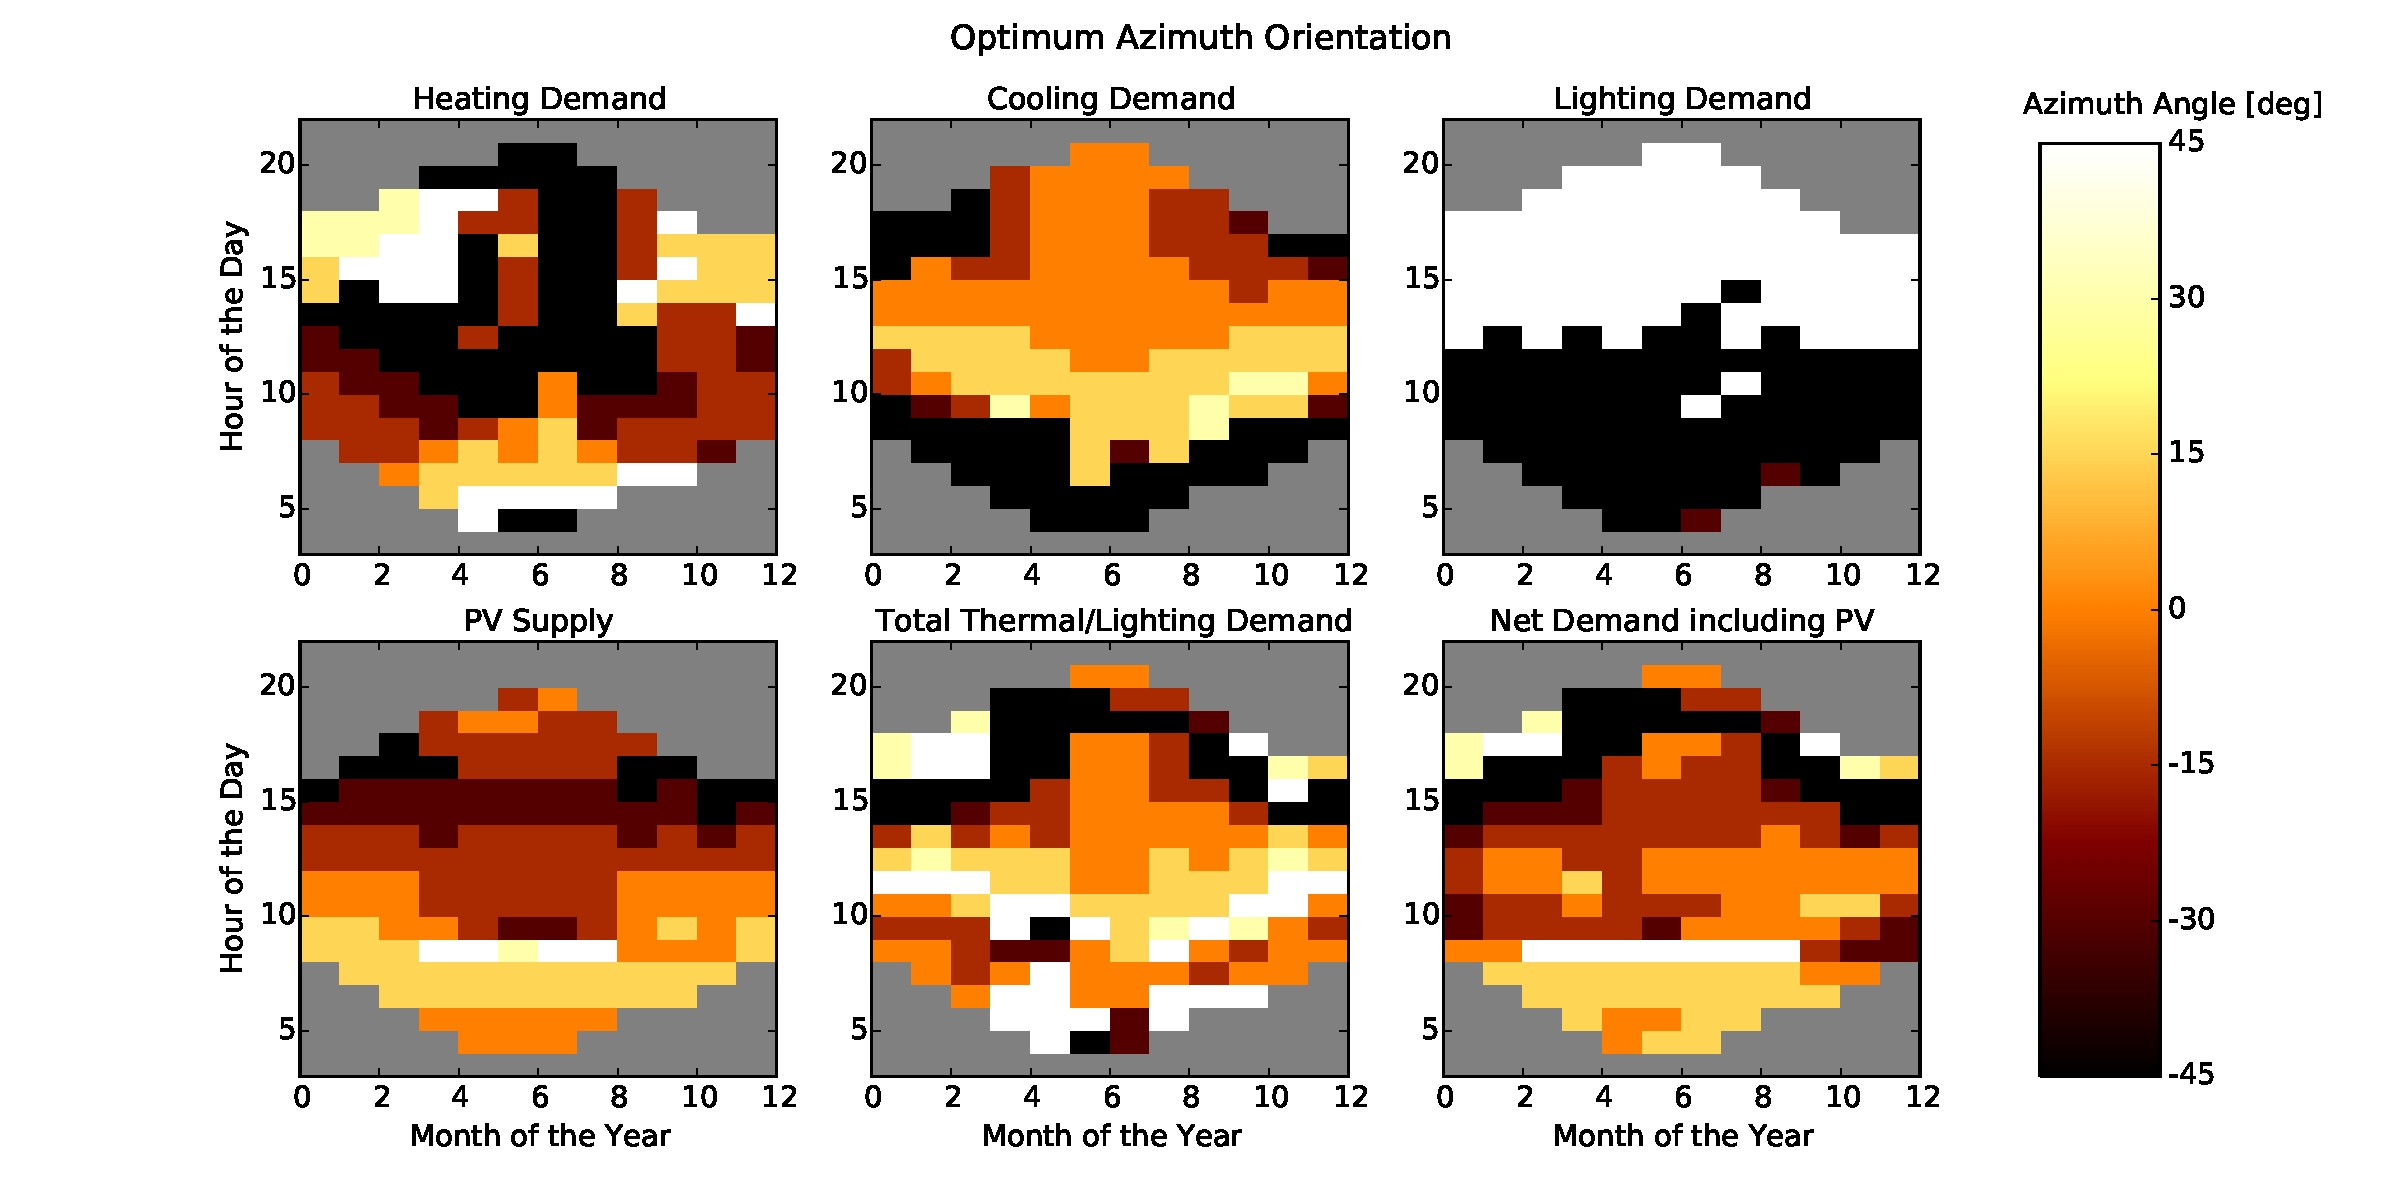
\includegraphics[width=\textwidth, trim= 0cm 0cm 0cm 0cm,clip]{monthly_azimuth}
	\caption{Carpet plots detailing the optimal azimuth configuration to minimise the (a) heating demand, (b) cooling demand, (c) lighting demand, and (d) maximise irradiance on PV panels. Each configuration is represented by an angle of orientation around the x-axis (Altitude) and y-axis (Azimuth) as seen in the legend. Figure (e) details the combinations for optimum building thermal management without PV production. (f) also includes the PV production}
	\label{fig:monthly_azimuth}
	\end{center}
\end{figure*}


	Figure \ref{fig:carpetplot_energy} shows the net energy use at these optimum angles. It is interesting to see how the combination of electricity generation and adaptive shading can compensate for the entire energy use during sunlit hours.

\begin{figure*}
	\begin{center}
	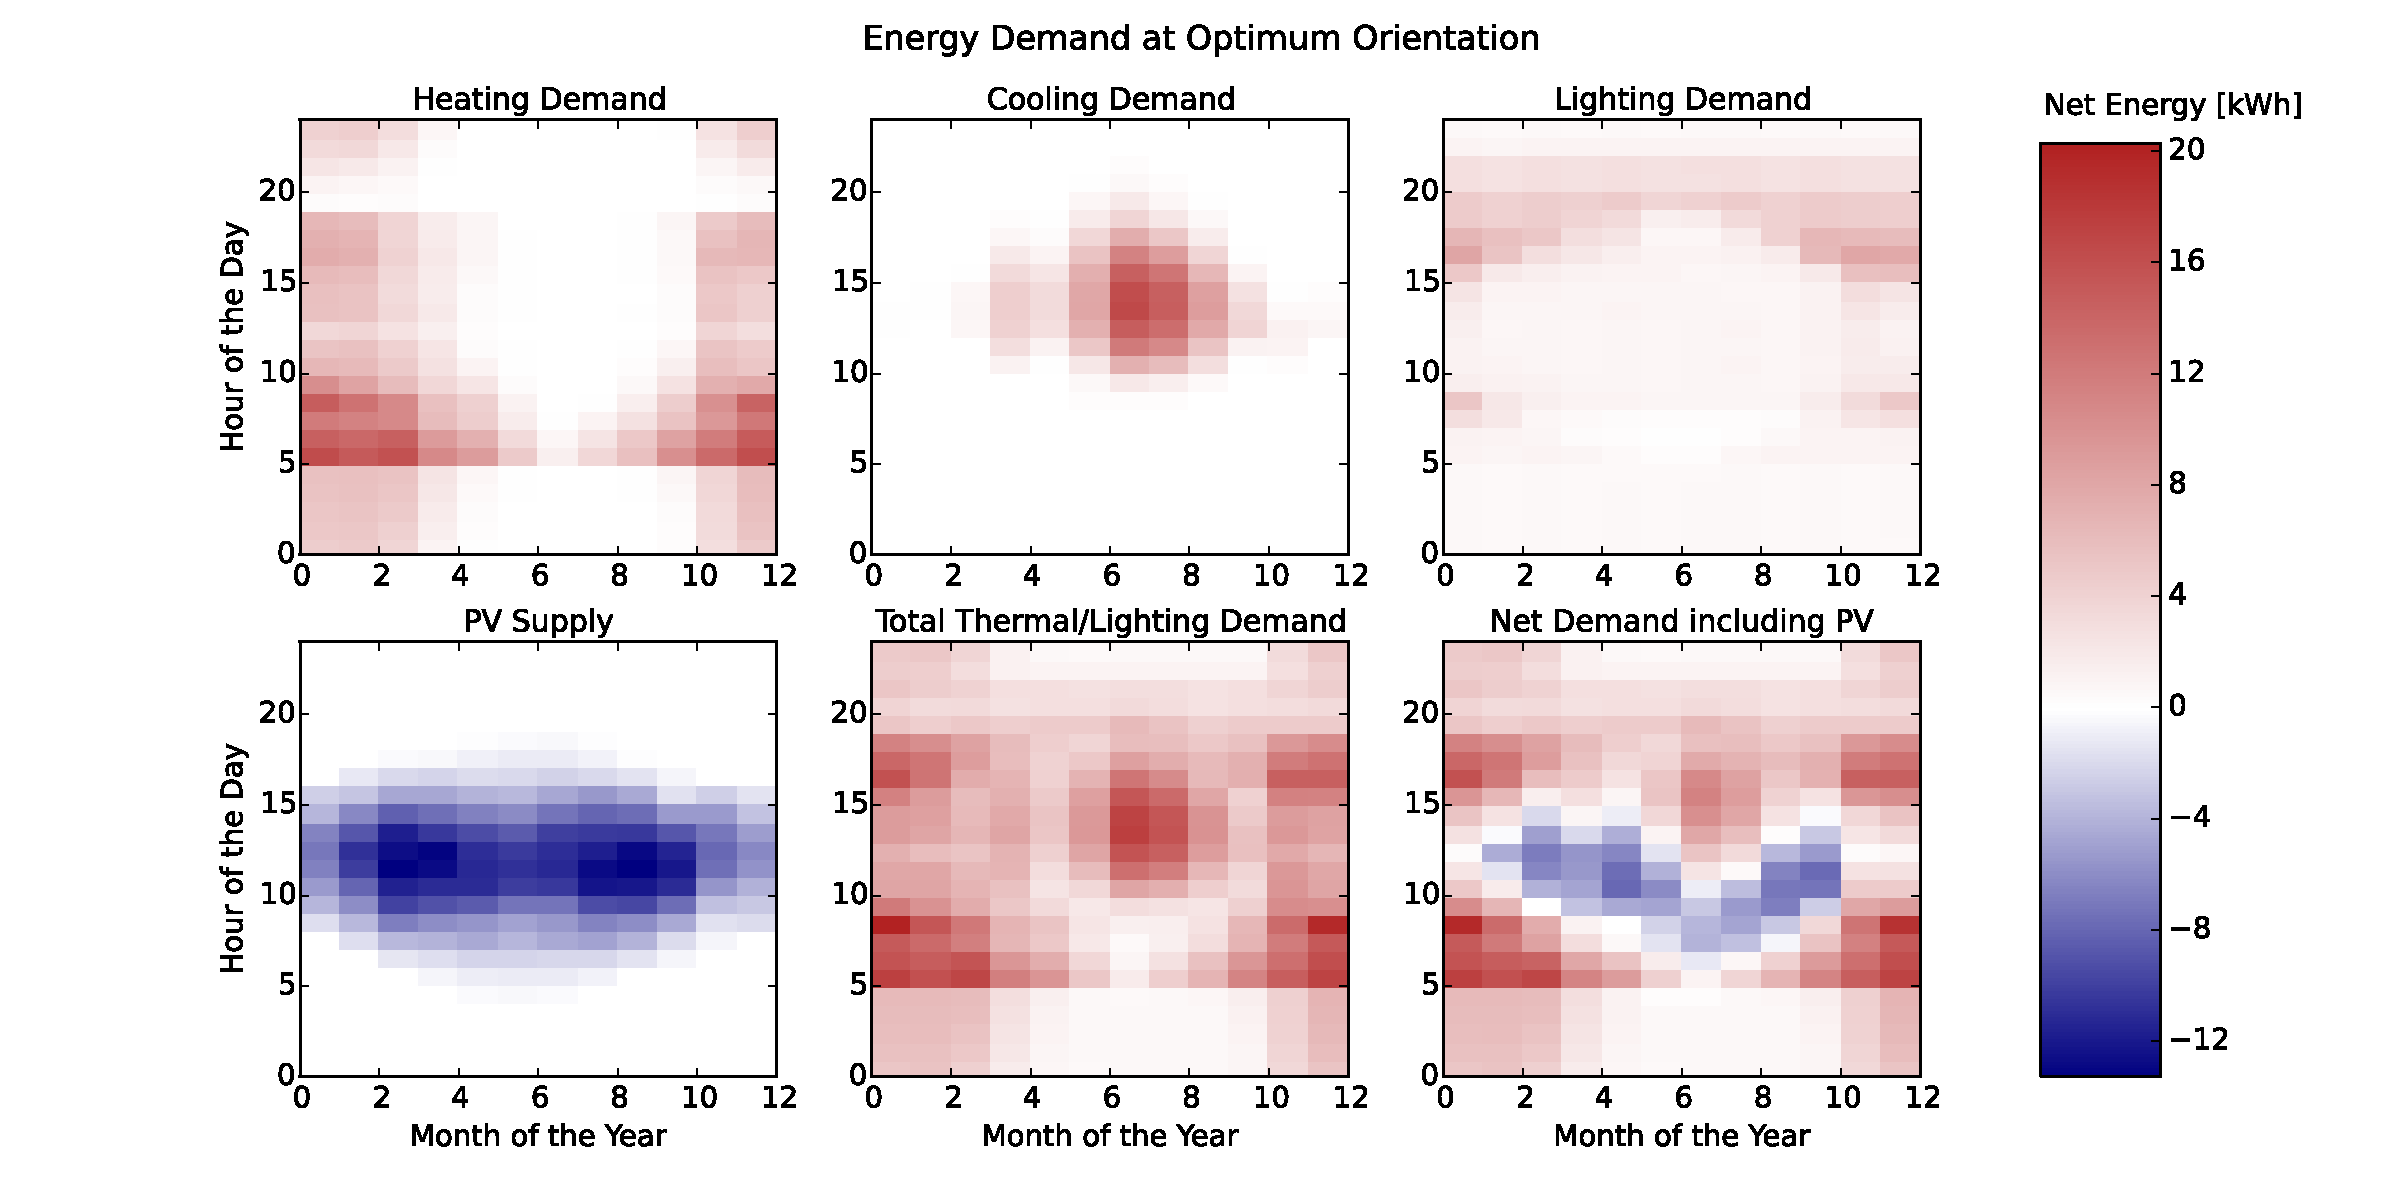
\includegraphics[width=\textwidth, trim= 0cm 0cm 0cm 0cm,clip]{monthly_energy}
	\caption{Carpet plots detailing the net energy consumption. Each square represents the total energy consumption for that specific hour of the entire month. Red colours detail the energy demand, while blue colours detail the energy supply.}
	\label{fig:carpetplot_energy}
	\end{center}
\end{figure*}


\section{Influence of Angle Actuation}
	In order to evaluate the influence of the actuation, three dimensional plots can be used to display all possible configurations and their corresponding energy benefit. In figure \ref{fig:3d}, the energy benefits of the altitude actuation can be seen for the months of March, June and September. Each plot displays one cumulative day in hourly resolution. The x-axis represents the hour of the day, the y-axis represents the altitude angles, and the z-axis represents the energy benefit of the actuation, i.e. the difference in energy usage between the evaluated angle and the angle that yields the worst overall energy usage for each hour. It can be seen that the energy benefit is by far the largest around noon. Furthermore, positions that are rather closed tend to have the highest influence for the said mid-day hours. Open positions normally yield the worst benefits, except for some early morning or evening hours, where heating and lighting become important. This overall behaviour corresponds well to the results depicted in figure \ref{fig:monthly_altitude}, and shows why the angles that yield the optimum total energy, generally match the angles that optimize cooling and PV electricity production. A further interesting observation that can be made from this figure is the non continuous curves for midday hours, at an altitude angle of around $30^{\circ}$, the energy benefit reduces over proportionally. This is caused by the PV electricity production, larger angles will increase longitudinal shading and therefore over proportionally reduce the energy yield. 

	\begin{figure*}
		\begin{center}
		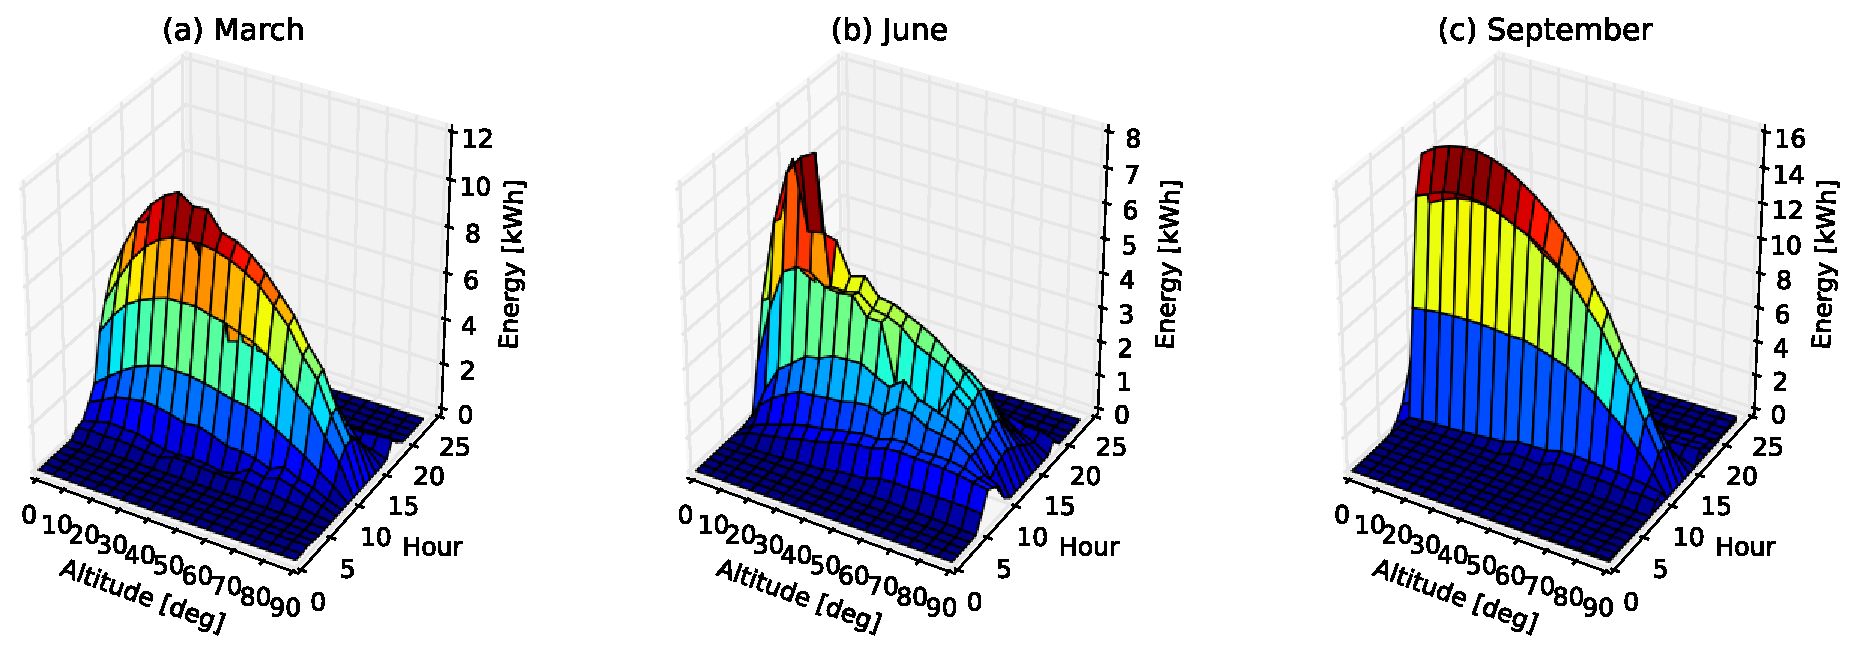
\includegraphics[width=1\textwidth, trim= 0cm 0cm 0cm 0cm,clip]{3d2}
		\caption{Energy benefits of the altitude actuation for the months of March, June and September. Each plot displays one cumulative day in hourly resolution. The x-axis represents the hour of the day, the y-axis represents the altitude angles, and the z-axis represents the energy benefit of the actuation, i.e. the difference in energy usage between the evaluated angle and the angle that yields the worst overall energy usage for each hour.}
		\label{fig:3d}
		\end{center}
	\end{figure*}


	
\section{Radiation and PV Analysis}

	
	To evaluate the performance of the radiation simulation, a grid-convergence study was performed and the optimum grid size for further simulations was found. The radiation results could then be used to calculate the PV electricity production, enabling the finding of optimum angles to maximize PV electricity production. The corresponding energy output was finally compared to a control strategy using solar tracking.

	%\subsection{Grid Convergence}

		%With a larger grid-size, results are less accurate. In order to study this effect, a grid convergence study was conducted. Figure \ref{f:gridConvergence} shows the grid size dependency of the total radiation on the asf. The colors in the first two plots on the upper left represent the hours of the day. One can see in the second plot - where the radiation is normalized by a division with the radiation for a grid-size of 12.5\,mm - that the results are significantly more accurate for morning and evening hours. This is caused by increased self-shading at midday hours. The colours in the third plot on the left show the dependency on different combinations. No clear pattern could be found here. Finally the average deviation is depicted in the fourth plot on the left and a box-plot with all deviations is shown on the right. It can be seen that a smaller grid-size leads to larger deviations. While for a grid-size of 400\,mm the average deviation is over 10\%, the deviation goes down to below 1\% for a grid size of 25\,mm. 25\,mm was therefore taken as the grid-size of all simulations, as it gives accurate results, while still being computationally feasible. 

		%\begin{figure*}
		%	\begin{center}
		%	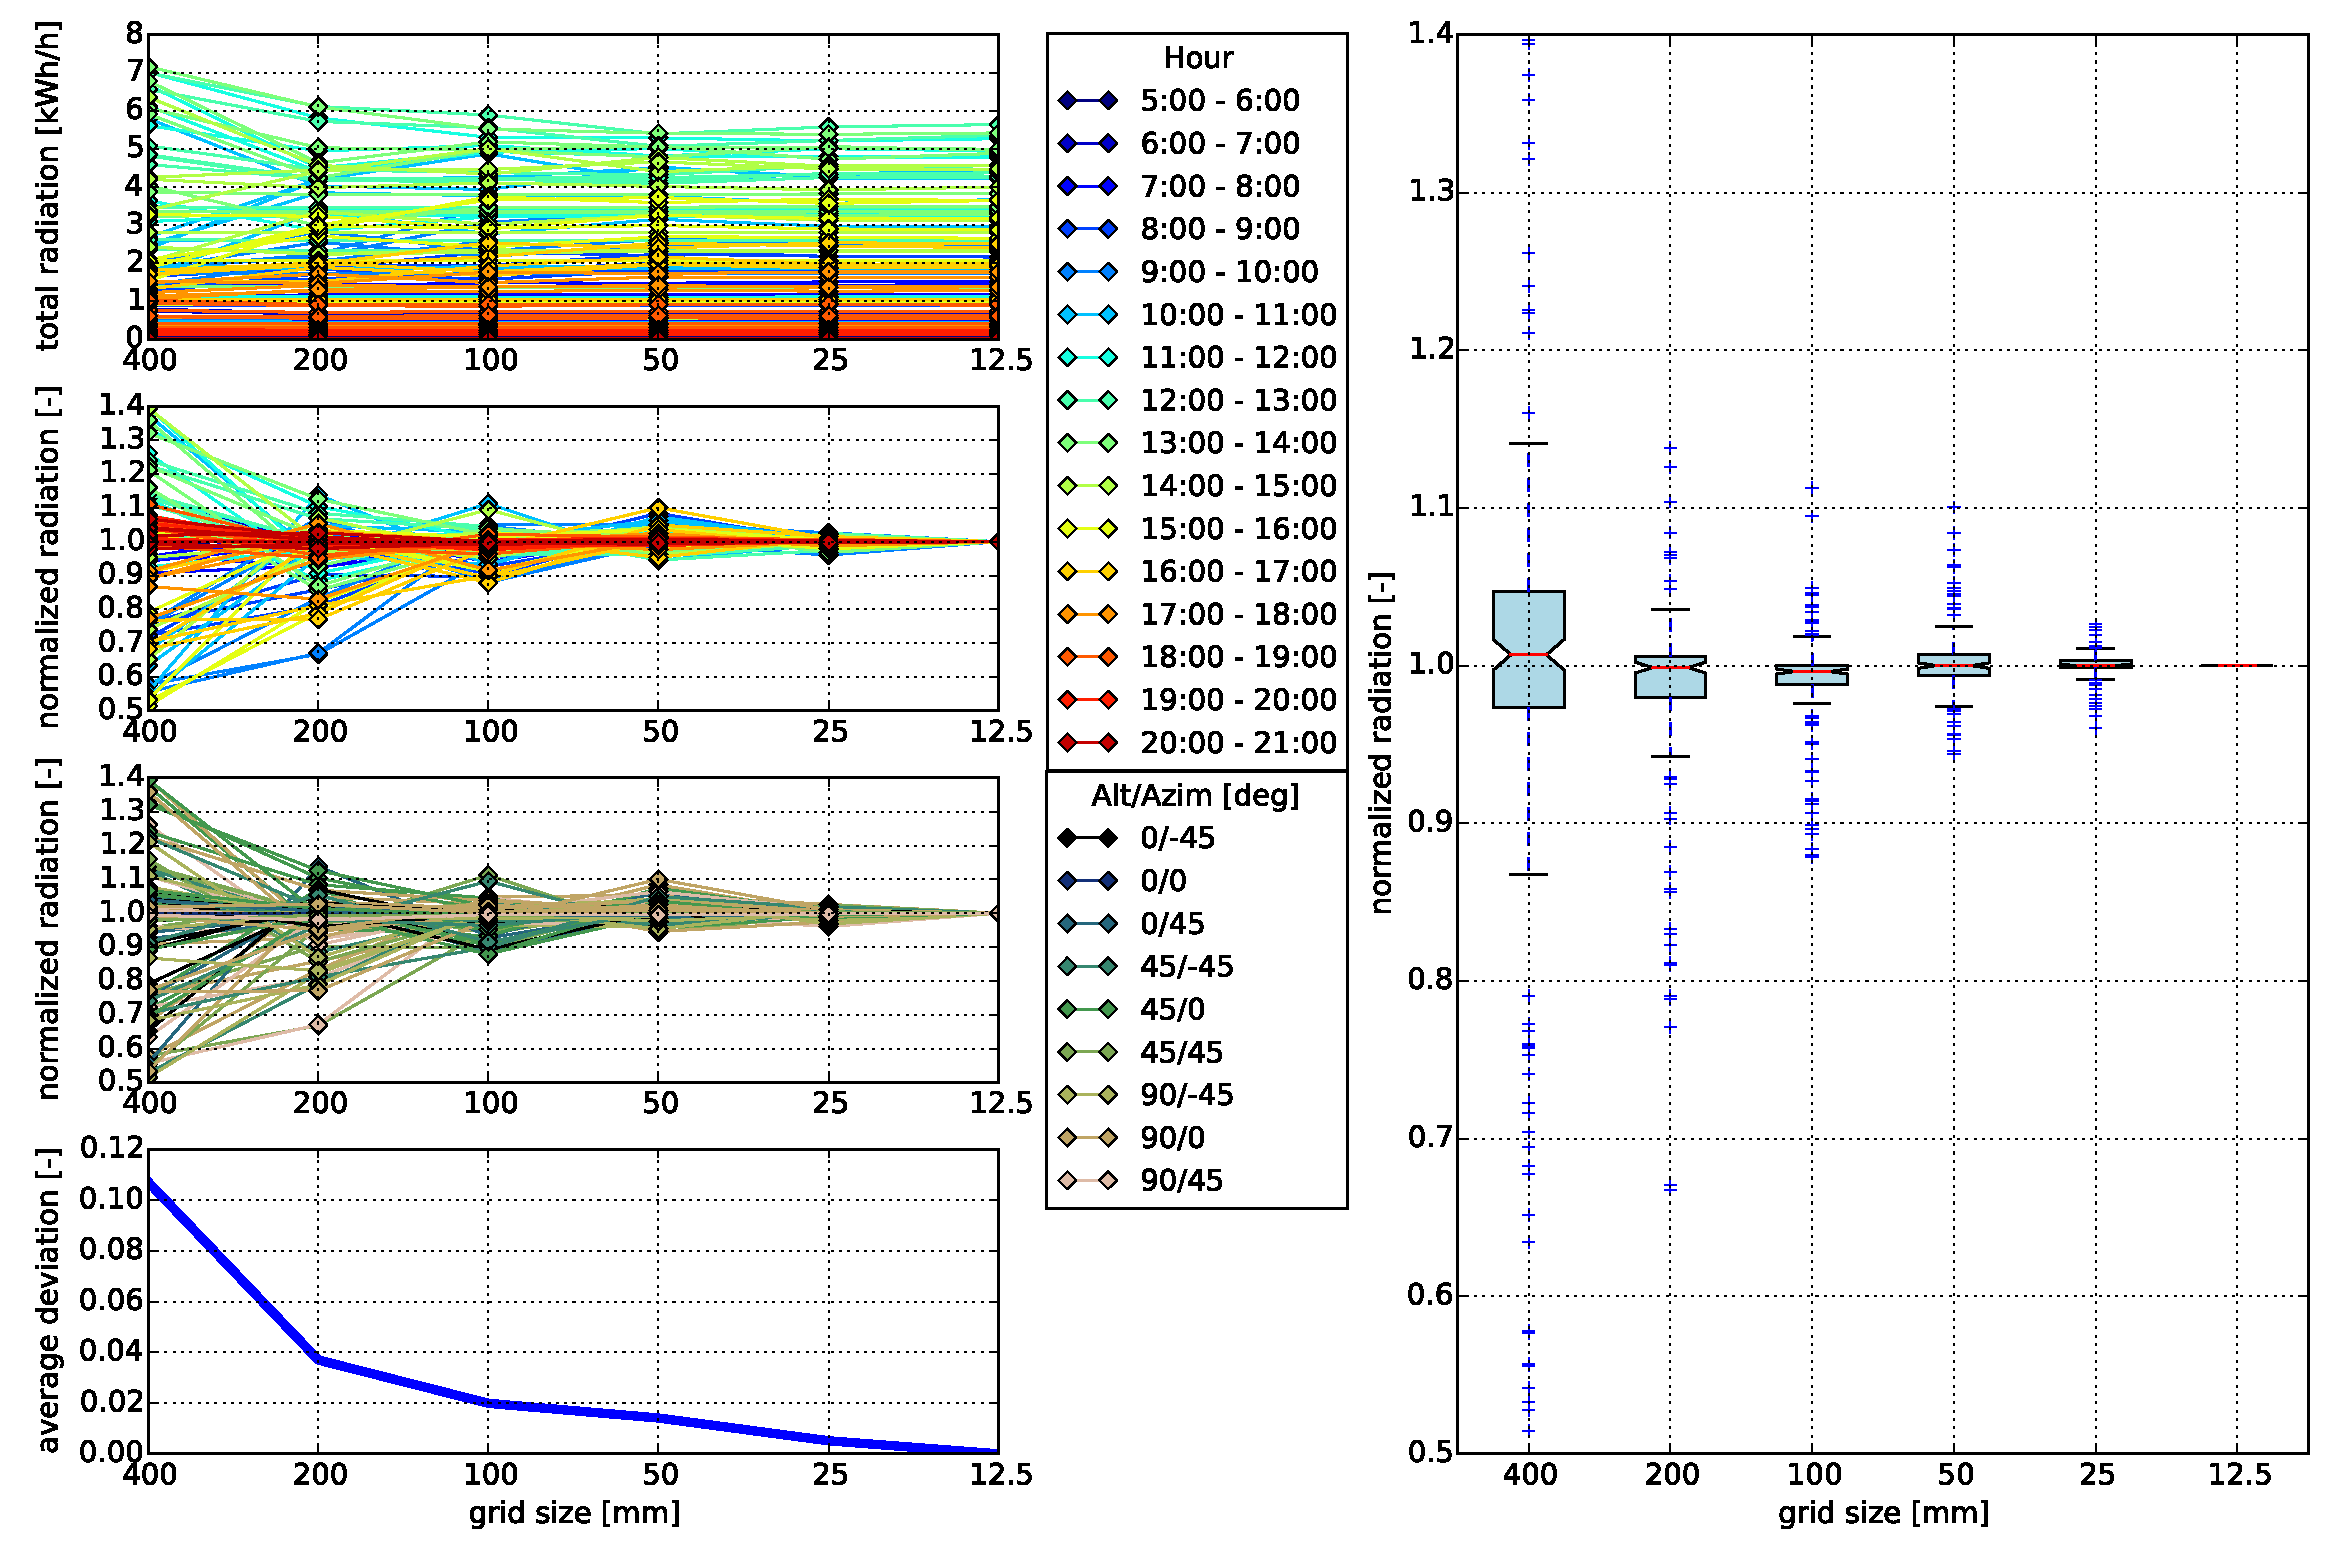
\includegraphics[width=\textwidth, trim= 0cm 0cm 0cm 0cm,clip]{gridConvergence.pdf}
		%	\caption{Grid convergence evaluation}
		%	\label{f:gridConvergence}
		%	\end{center}
		%\end{figure*}

	\subsection{Comparison of Sun Tracking to Optimized Solution}
	\label{ss:compareSunTracking}

		In order to evaluate the optimum configuration for PV production, simulations using sun-tracking were compared to simulations evaluating 49 different combinations (i.e. 7 different azimuth and altitude angles). Figure \ref{f:compareSuntracking} shows the radiation on the panels in the first plot, also comparing it to the maximum radiation. The second plot shows the PV electricity production for the two different control strategies, whereas the third plot compares the corresponding efficiencies. It can be seen that while the radiation on the panels is pretty similar for both sun tracking and the optimized solution, the PV electricity production of the optimized solution is significantly higher than the sun-tracking solution in the afternoon hours. This is caused by the layout of the PV panels, longitudinal shading causes high power losses \cite{hofer2015PVSEC}, thus the optimized solution decreases the longitudinal shading compared to sun-tracking. 

		\begin{figure*}
			\begin{center}
			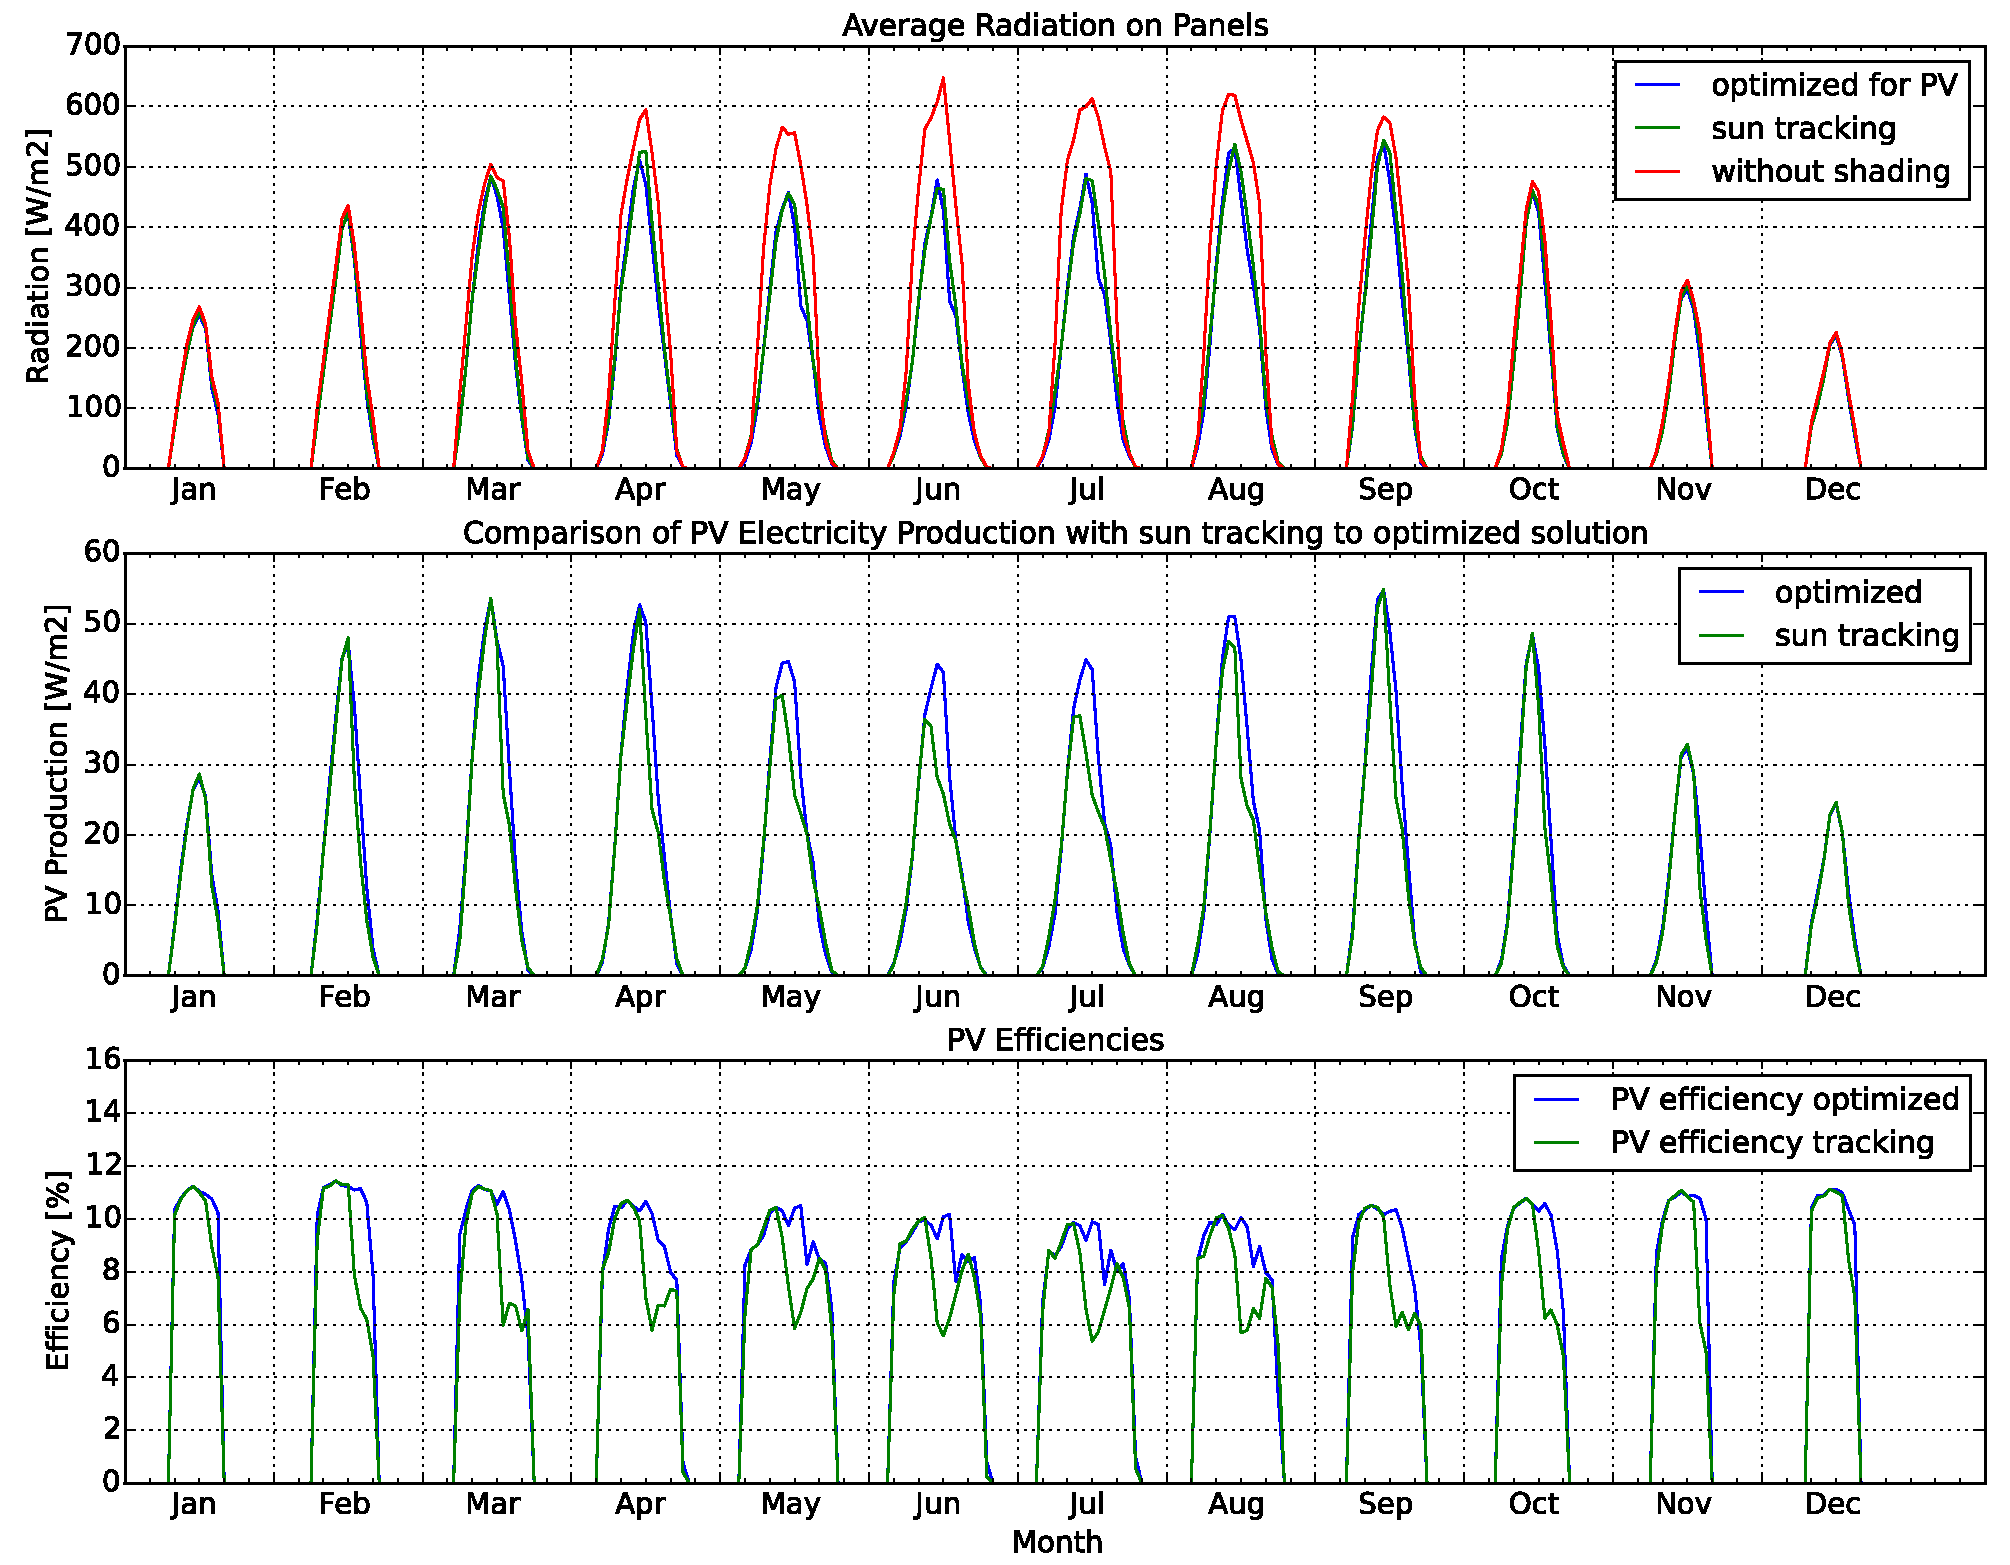
\includegraphics[width=\textwidth, trim= 0cm 0cm 0cm 0cm,clip]{PV}
			\caption{Comparison of optimized solution to sun-tracking. a) average radiation on panels compared to radiation without shading b) PV electricity production comparison c) efficiency comparison}
			\label{f:compareSuntracking}
			\end{center}
		\end{figure*}






\section{Orientation Analysis}

	Evaluations of the facade for different building orientations were done with the basecase of 5 azimuth and 5 altitude angles. Non surprisingly, the south facing facade produces the most electricity and has therefore the lowest net energy as can be seen in figure \ref{fig:buildingOrientation}. It was found that the PV apertures should be oriented parallel to the upper left edge for facades that are west or south-west oriented, whereas they should be oriented parallel to the upper right edge for east or south-east oriented facades. This is caused by the shading patterns, longitudinal shading needs to be prevented as described in section \ref{ss:compareSunTracking}. An east facing facade uses less heating compared to a west facing facade, as heating is most important during morning hours. For similar reasoning the east facing facade needs more cooling energy than the west facing facade, because the room heats up in the morning. Interestingly, PV production is higher for the west facing facade than for the east facing facade. The cause for this is probably because of conflicts in optimizing cooling and PV electricity production at the same time, as cooling is more dominant for the east facing facade. 

	\begin{figure*}
	\begin{center}
	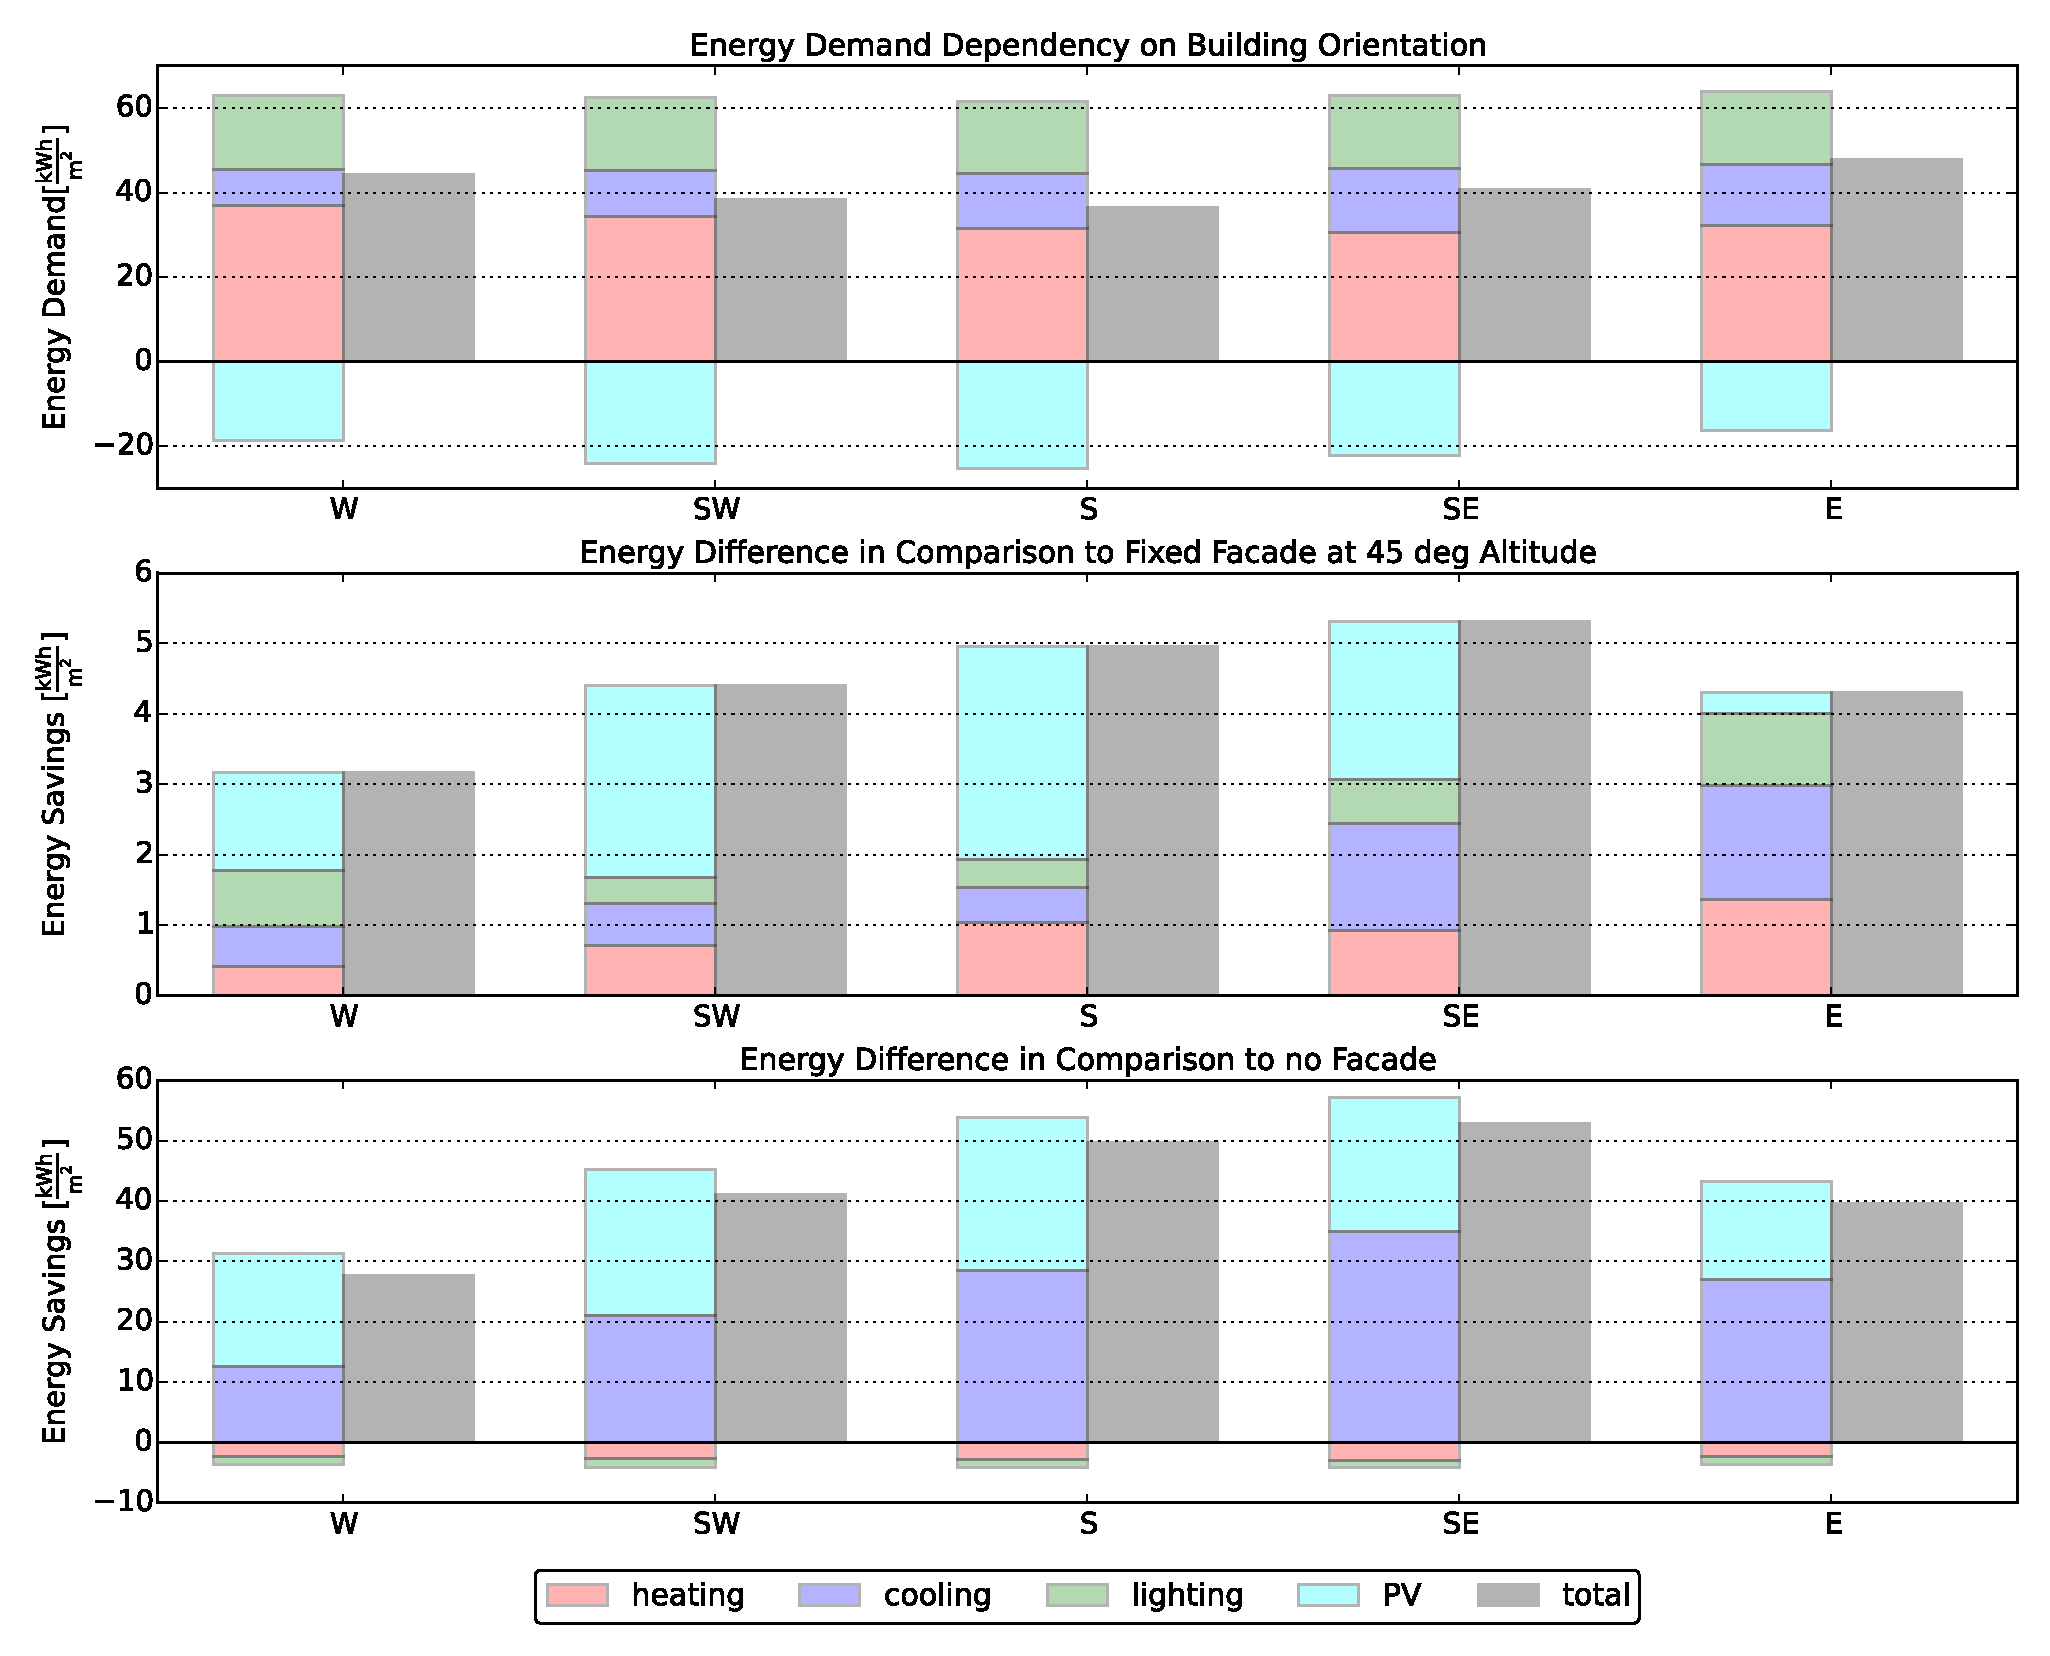
\includegraphics[width=\textwidth, trim= 0cm 0cm 0cm 0cm,clip]{orientation}
	\caption{Energy demand in dependence of building orientation. South facing facades perform best.}
	\label{fig:buildingOrientation}
	\end{center}
	\end{figure*}

\section{Sensitivity Analysis}

	A sensitivity analysis was done for heating COP, cooling COP, lighting load, average PV efficiency, building orientation, infiltration rate and combination variations for the time period of one year. The results are shown in figure \ref{fig:sensitivity}. The top row shows the energy savings per square meter of room area compared to a fixed solare facade at an angle of 45\degree, whereas the bottom row shows the energy savings compared to a building without any PV modules or shading devices. 

	\begin{figure*}
	\begin{center}
	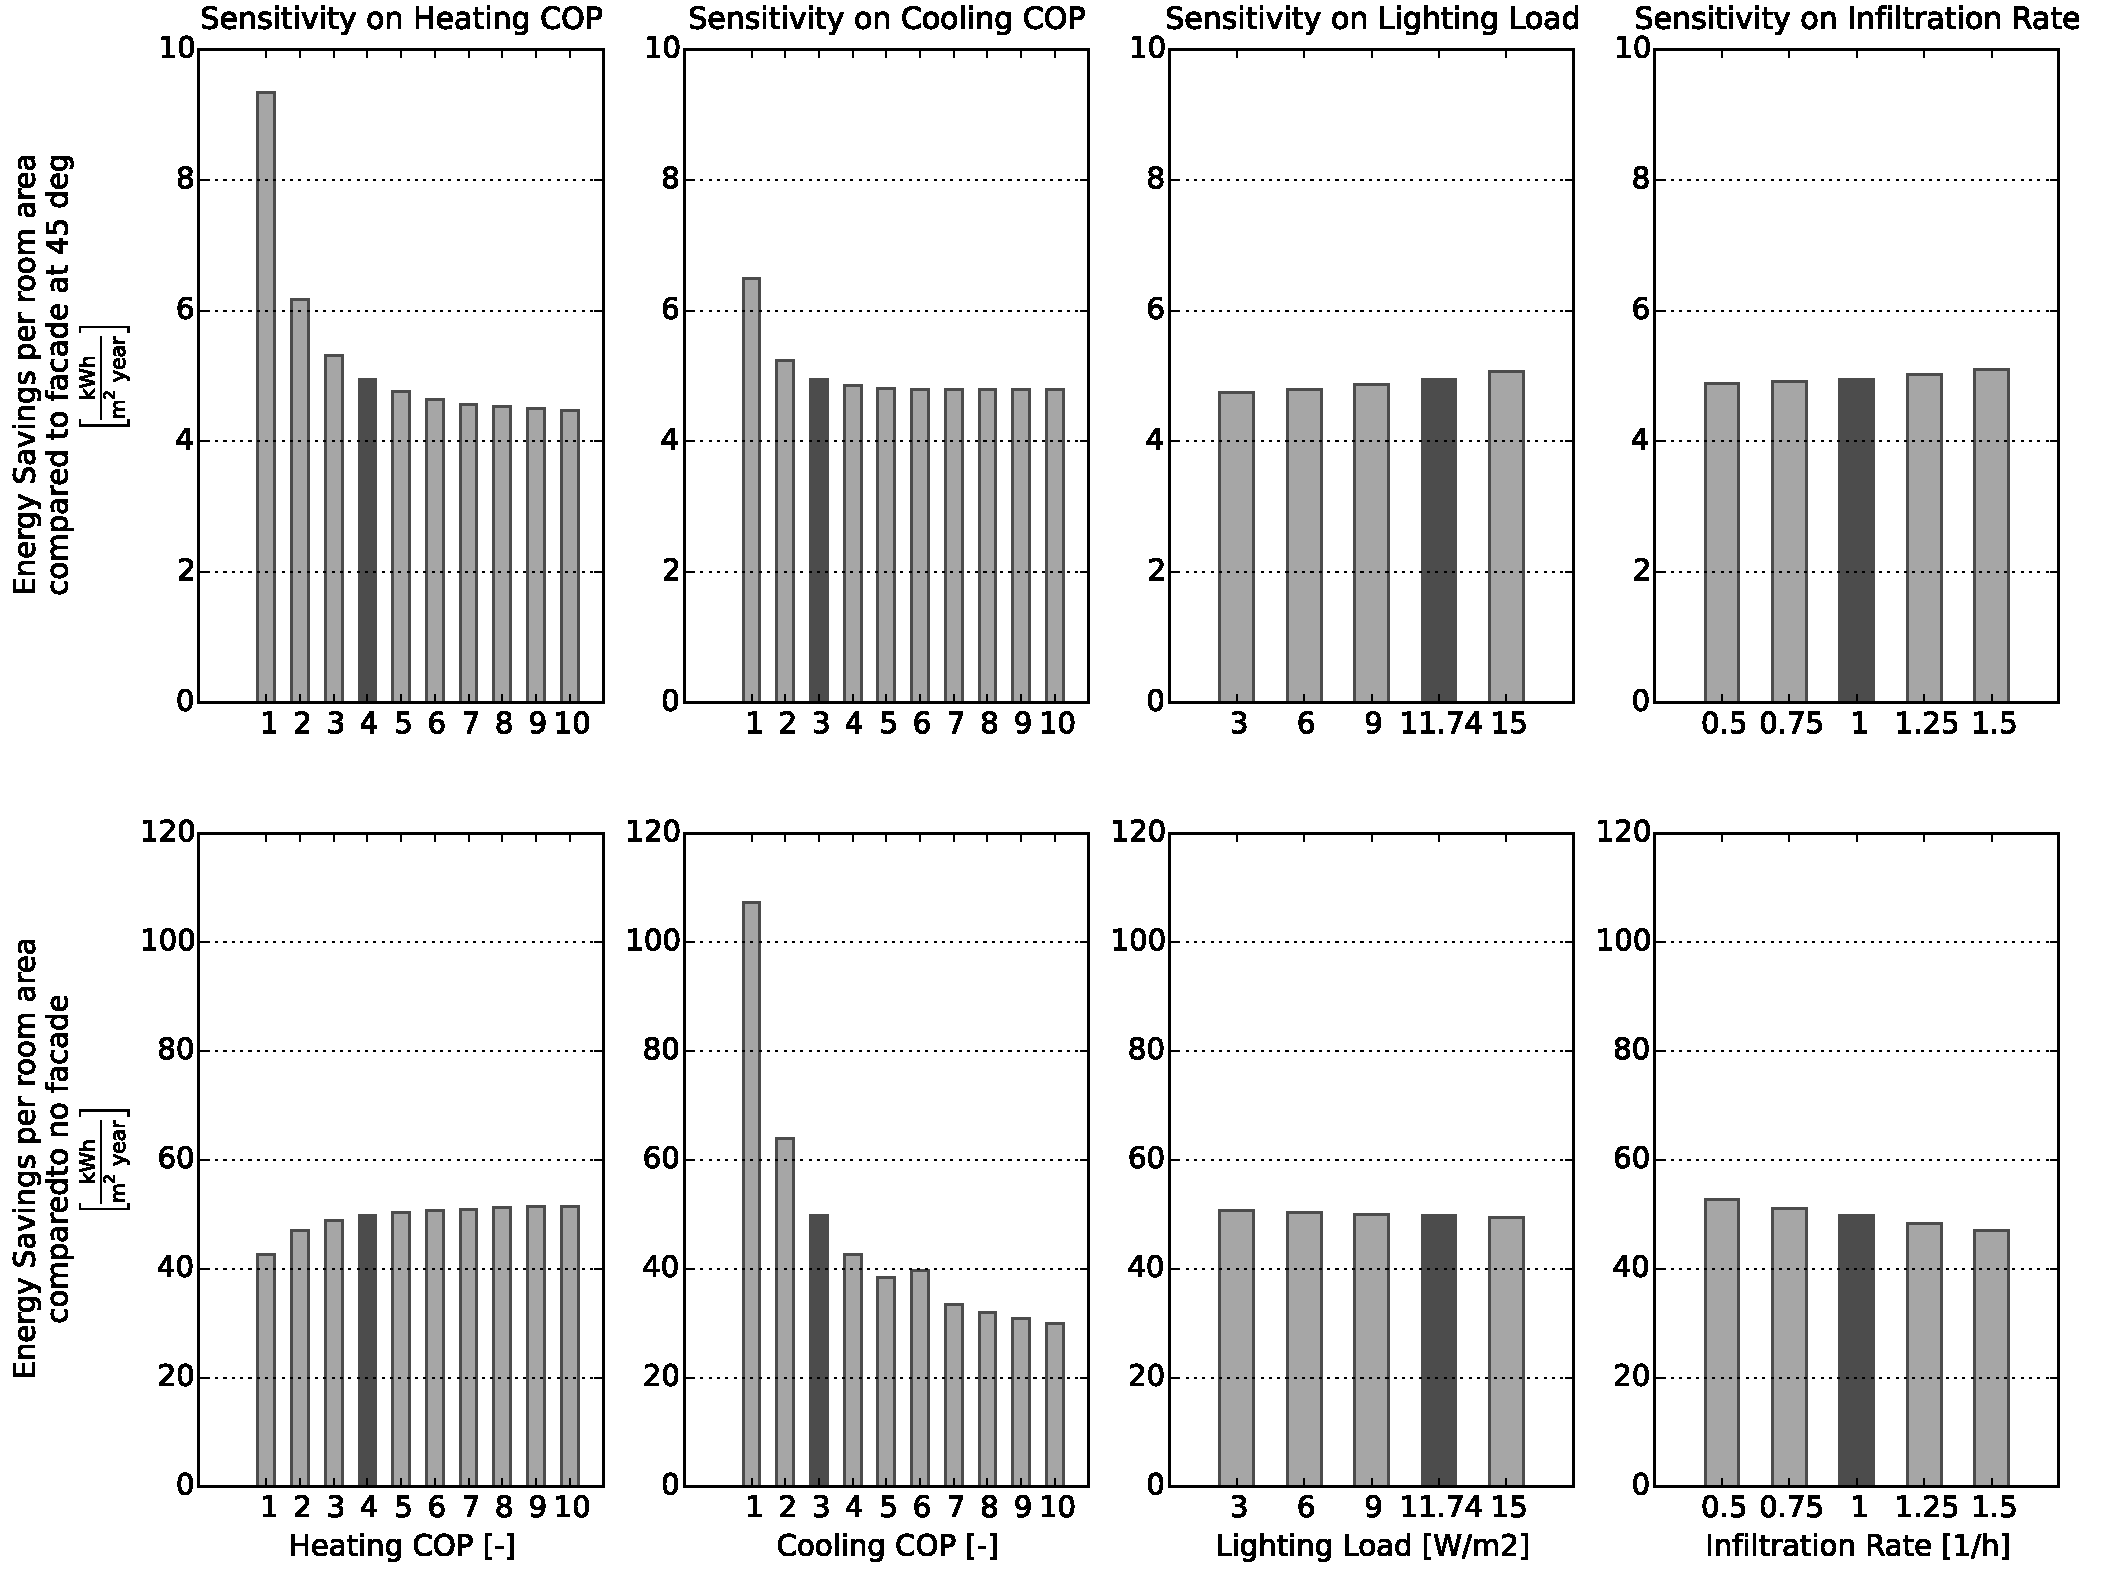
\includegraphics[width=\textwidth, trim= 0cm 0cm 0cm 0cm,clip]{buildingSensitivity}
	\caption{Sensitivity analysis of energy savings during one year. From left to right, sensitivities on heating COP, cooling COP, lighting load, average PV efficiency, building orientation, combination variations and infiltration rate. Top row shows the energy savings compared to a fixed solar facade at a 45\degree altitude angle, the bottom row shows the energy savings compared to a room without shading or PV modules.}
	\label{fig:sensitivity}
	\end{center}
	\end{figure*}

\section{Potential of Individual Actuation}
	Individual actuation of the panels is one of the key advantages of the ASF that have to be closely evaluated. In order to quantize the potential of individual actuation, evaluations were performed by splitting the ASF into clusters. Due to computational limitations, especially on the radiation part, simplified geometries were used for the radiation evaluation, using only ten panels in four rows with two clusters and eight panels in three rows with three clusters, rather than the 50 panels of the reference case with one cluster. Furthermore only the months of March, June, September and December were evaluated. The two cluster evaluation was done for the reference case with five azimuth and five altitude angles. The evaluations with three clusters was done only for altitude variations, with 5 angles in each cluster. The simulations showed promising results, in the two cluster case, the total energy demand could be reduced by one percent, whereas for three clusters, the total energy demand was reduced by 5 percent. 